\documentclass[10pt]{article}
\usepackage[utf8]{inputenc}
\usepackage{listings}
\usepackage{float}
\usepackage{graphicx}
\usepackage{fullpage}
\usepackage{caption}
\usepackage{subcaption}
\usepackage{amsmath}
\usepackage{hyperref}
\usepackage{epstopdf}

%\renewcommand{\thesubsection}{\arabic{subsection}}
\renewcommand{\thesubsubsection}{\alph{subsubsection}}

\title{Signals and Systems Lab 1}
\author{Maikel Withagen (s1867733) \and Steven Bosch (s1861948)}
\date{\today}
\lstset{
frame=single,
numbers=left,
breaklines=true,
language=Matlab,
basicstyle=\footnotesize,
title=\lstname,
showstringspaces=false
}

\renewcommand{\thesubsection}{\small(\alph{subsection})}
\begin{document}
\maketitle

\section{Summing Sinusoids}
\subsection{a}
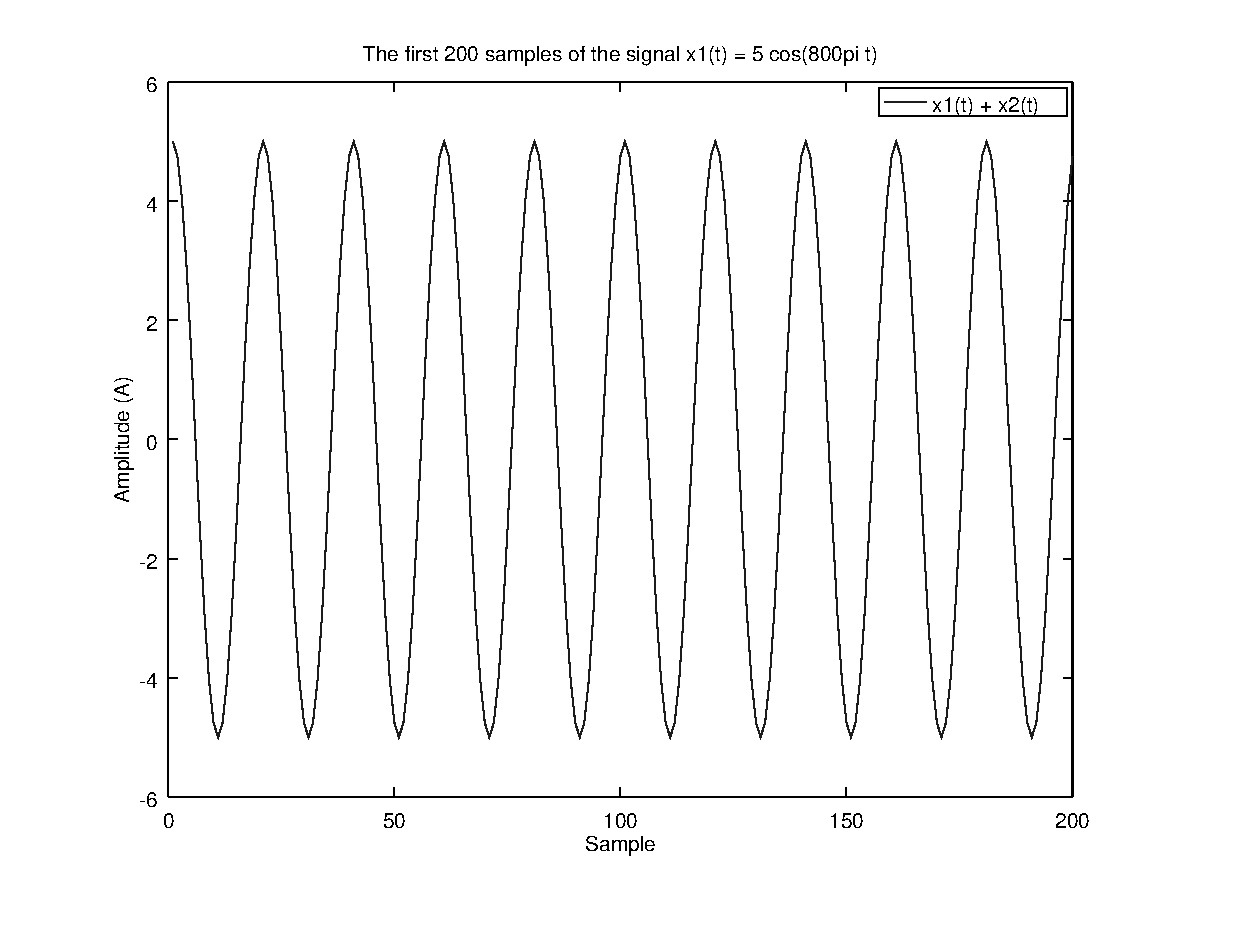
\includegraphics[width=\columnwidth]{plot1A.eps}
\subsection{b}
\subsection{c}
\subsection{d}
The shift of $0.013125s$ translates to a period of $\omega * t = 800\pi*0.013125 = 10.5\pi$.
Now we got the following formulas:
\begin{equation}
    x1(t) = 5 cos(800\pi t)
\end{equation}
\begin{equation}
    x2(t) = 5 cos(800\pi t + 10.5\:pi)
\end{equation}
Now we can generate x1(t)+x2(t) by using our created function gensinusoid.\\
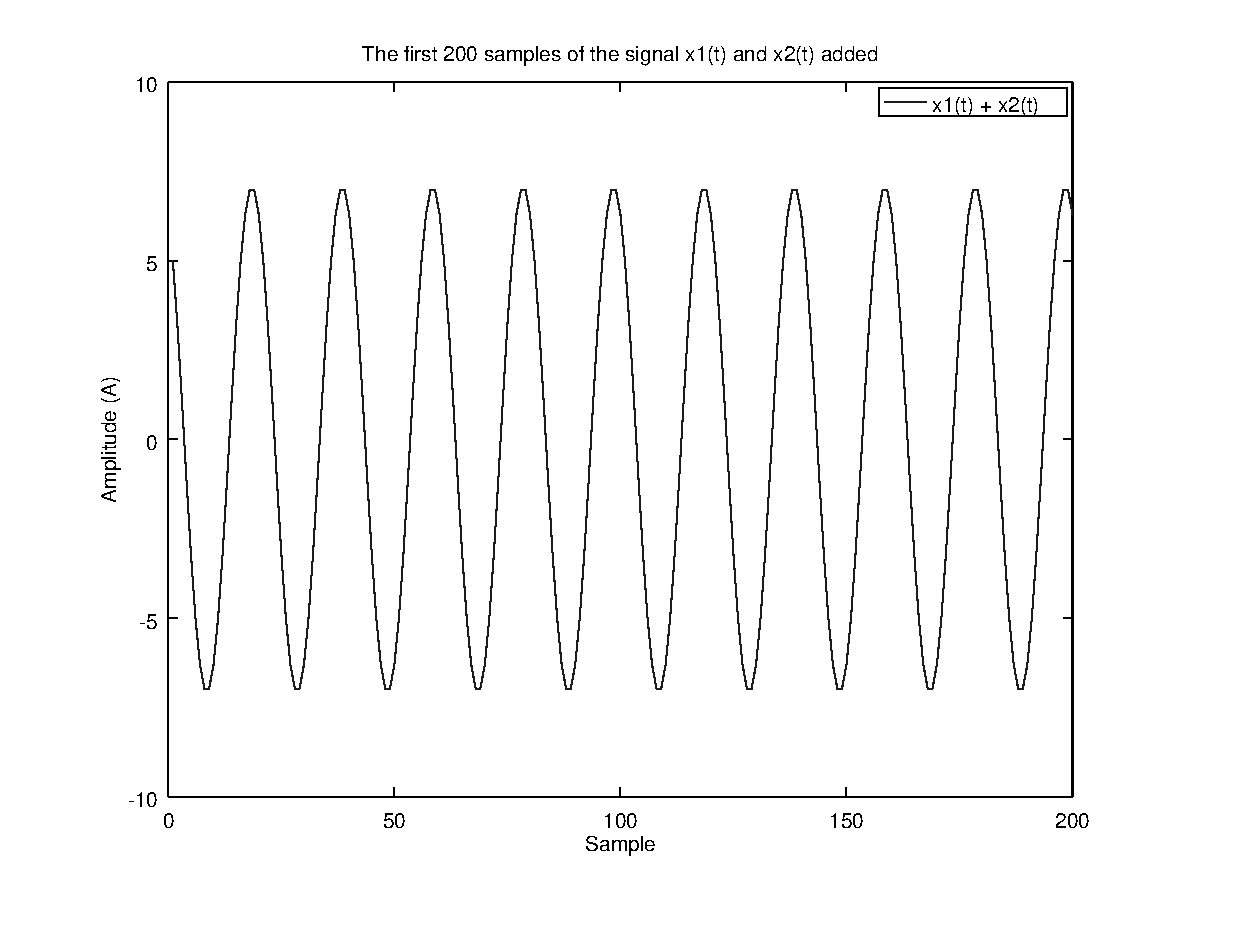
\includegraphics[width=\columnwidth]{plot4A.eps}\\
Using the sumsinusoid function we can calculate the values for y(t):
$[A, f, phi] = 7.07107,400.00000,0.78540$, giving us\
\begin{equation}
    y(t) = 7.07107 cos(400*2*\pi t + 0.78540)
\end{equation}
The plot with both lines shows a perfect overlap,
so we can conclude that our answer for y(t) is correct.
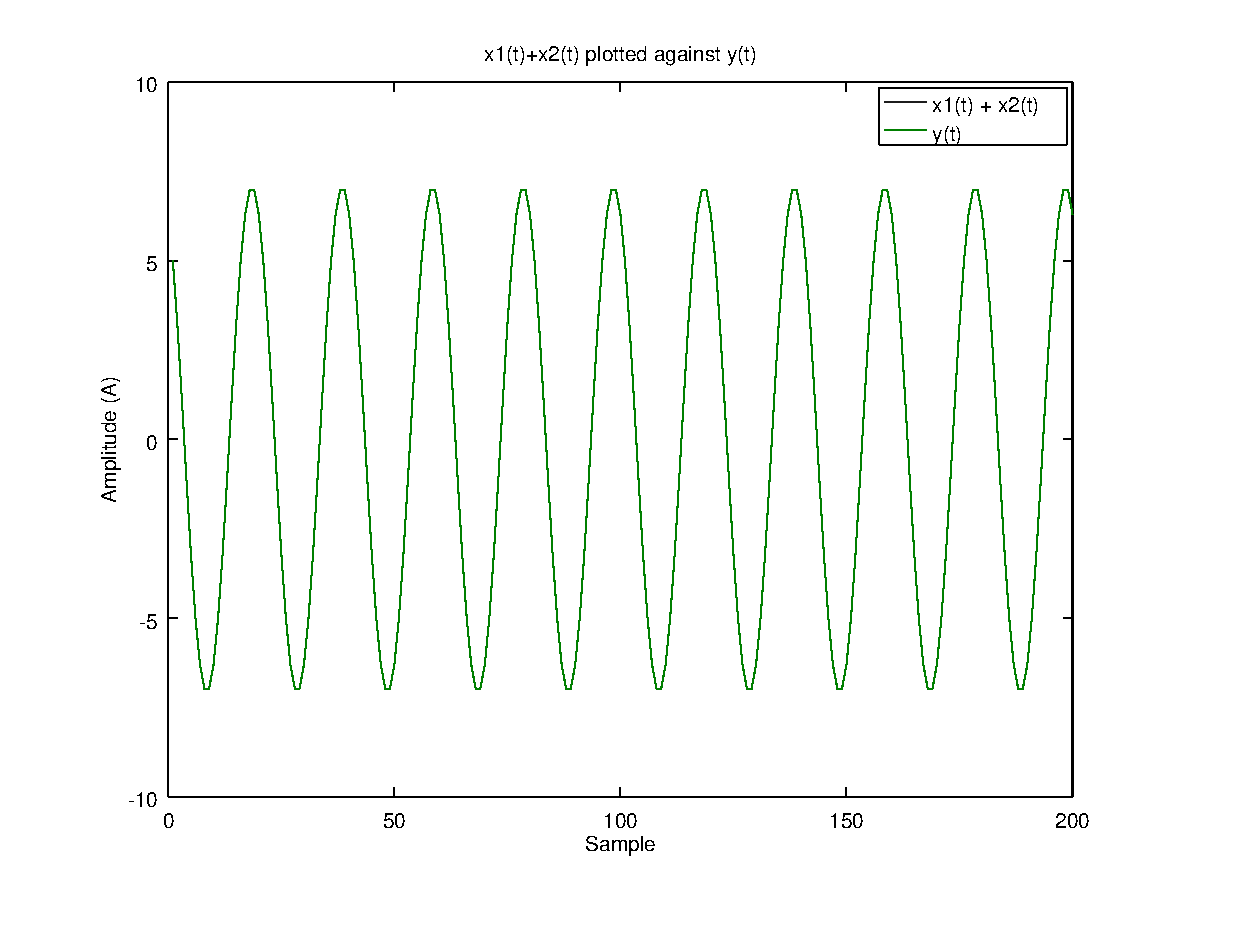
\includegraphics[width=\columnwidth]{plot4B.eps}

\subsection{e}


\newpage
\section*{Appendix}
\appendix
\section{Summing Sinosoids}
%\lstinputlisting{../Code/kmeans.m}{\label{kmeans}}


\end{document}
